% !TeX root = ../report.tex

\section{Feature based approach}\label{sec:feature}

For the feature based approach, a feature extraction is done with regards to the term frequency - inverse document frequency. This has been the golden standard for feature extraction, and ensures that the features extracted have the highest descriptive effect with regards to the tweets in which the feature occurs versus the tweets in which the feature does not. These extracted features are then used for the training of one of two different models, depending on the subtask at hand.\\
Both models build on the random forest learning method since its properties support both regression and multi-label classification. \\
The two models share the same general feature extraction, so they can be made directly comparable if the extraction parameters are kept comparatively the same.

\subsection{Custom features} \label{sec:customfeat}
Besides the Tf-idf feature extraction method, the model uses a custom feature extraction function. This function has different flags, corresponding to different features that could be of interest in these particular tweets. \\
These different custom features involves e.g. whether or not a hashtag is present or if the spelling error of the whole tweet is above some threshold. All of these custom features are boolean values in the sense that they are either present or not. The features are:\\
\begin{itemize}
\item Exclamation: check whether or not an exclamation mark was present in the tweet.
\item Hashtag: check whether or not an hashtag was present in the tweet.
\item Spelling: check whether or not are specified percentage of the tweet was mispelled.
\item Negative emoji: check whether or not an emoji from a list of negative emojis was present in the tweet.
\item Positive emoji: check whether or not an emoji from a list of positive emojis was present in the tweet.
\item Emoji: check whether or not an emoji was present in the tweet.
\end{itemize}
These features are then appended to the feature matrix returned by the Tf-idf extraction function, so that they are taken into consideration when training the different models. \\
Custom features can be based on linguistic and contextual intuition as well as a higher degree of linguistic analysis, as opposed to the deep learning features which will be trained with a more mathematically and statistical paradigm in mind.

\subsection{Model overview}
All the models share the same feature extraction method and the actual models were implemented using libraries which allowed a very high level approach. This acted as an introduction to the subtasks and which ones would be interesting to focus on and also as a baseline system which would work as a stepstone for the deep learning models used later in the process. In the final version of the code, two feature based models were used:\\
\begin{itemize}
 \item Random forest classifier
 \item Random forest regressor
\end{itemize}

\subsection{Hyperparameter testing}
\subsubsection{Regression, task 1}
HUSK AT ÆNDRE DET HER DA VI PRØVER ALLE CUSTOM FEATURES\\
Figure \ref{fig:max_f_ngram15_hashtag} is a plot of the Pearson score with regards to the amount of max features used in the final feature based model to solve task 1. This model all six single custom features. Furthermore, an n-gram range of 1 to 5 was used in the model.
\begin{figure}[H]
    \centering
        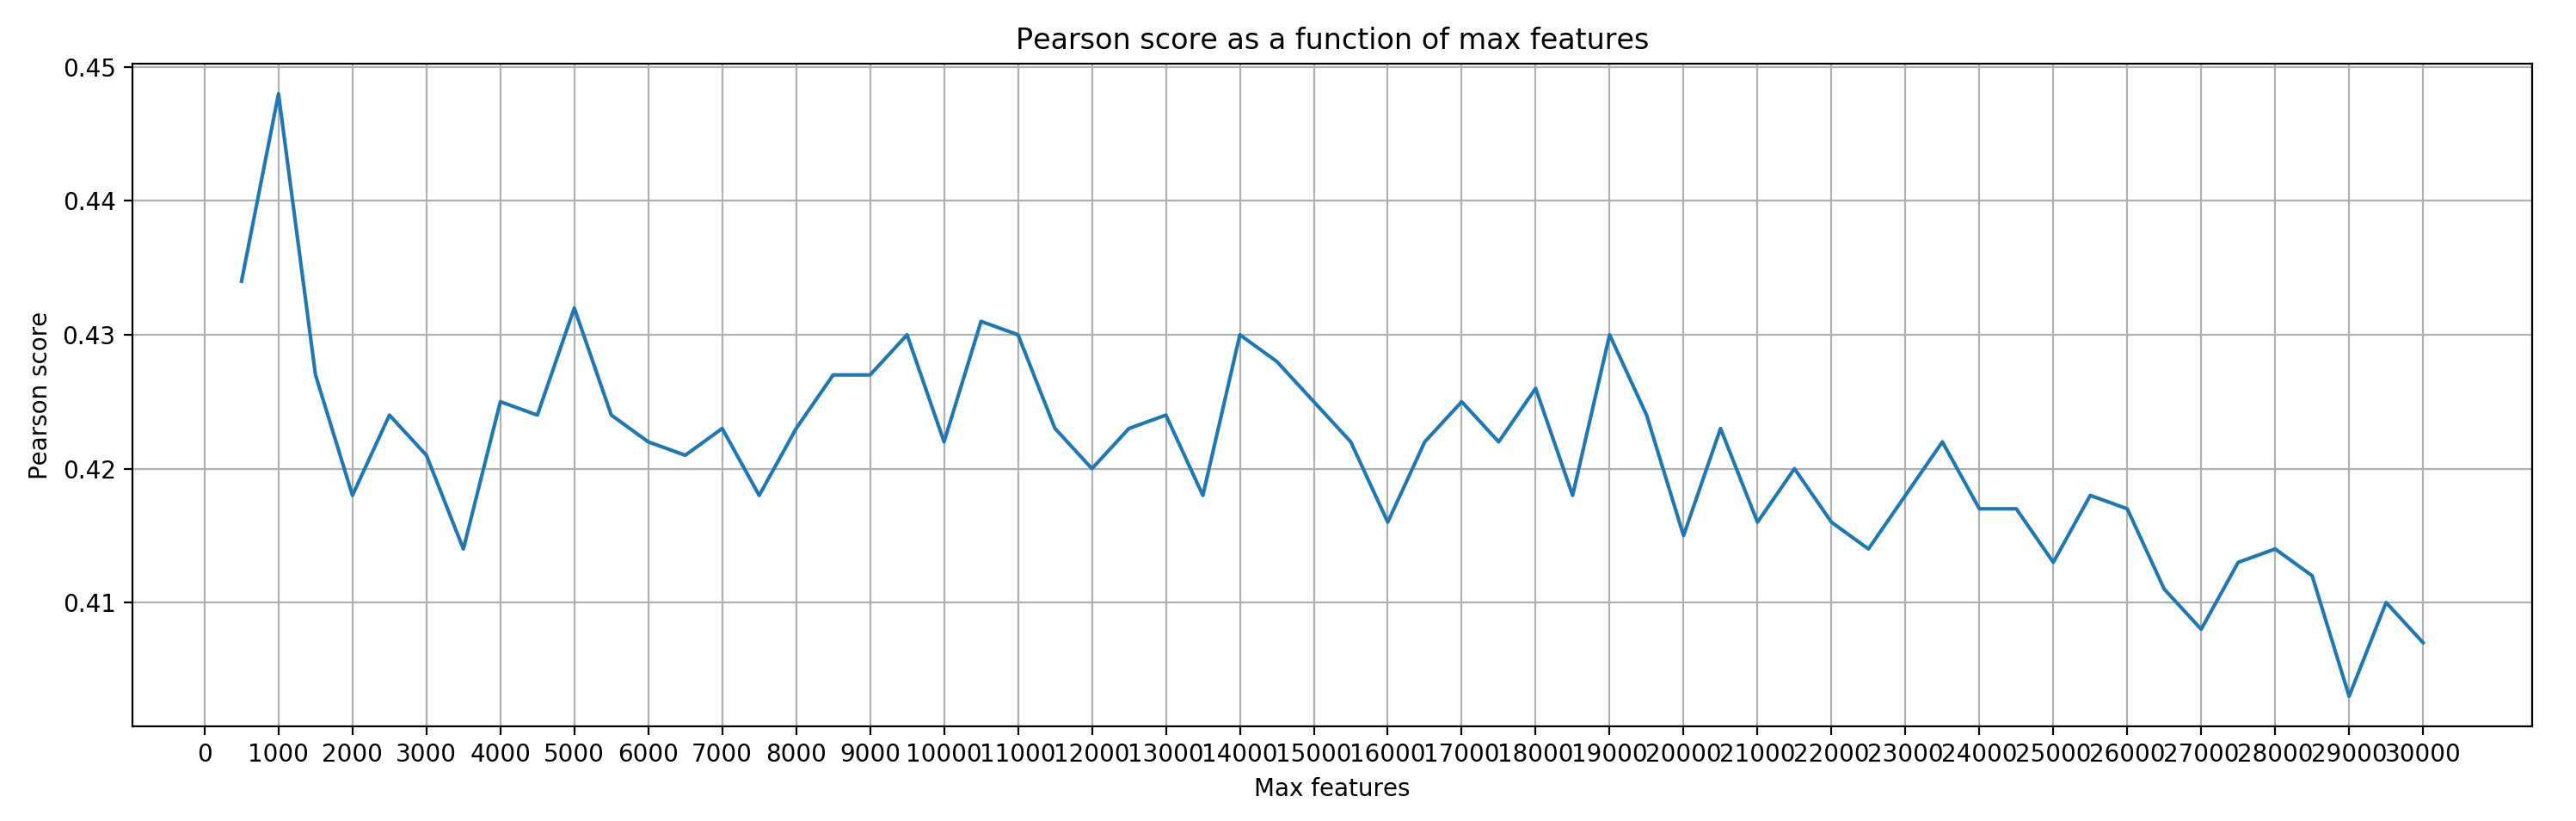
\includegraphics[width=\textwidth]{pictures/max_f_pearson.png}
        \caption{Pearson score as a function of max-features from 500-30000 with n-gram range 1-5 and all the custom features on}
        \label{fig:max_f_pearson}
\end{figure}
It is evident from figure \ref{fig:max_f_ngram15_hashtag} that there is not clear-cut correlation between the max features and the Pearson score. The tests were run with up to 30000 max features (results can be seen in appendix HUSK EN REF), but after 10000 features there was a steady drop off in the Pearson score.\\
\\
The use of n-grams in tweets was also complicated. Since the tweets are so dense and diverse, larger n-grams have very little chance of reappearing in other tweets, and as such there was very little difference in the n-gram ranges used when the max features was kept in place. The results of testing this is shown in table \ref{tab:ngram}\\
\begin{table}[h]
\centering
\begin{tabular}{c|c|c|c|c|c}
N-gram range & \text{Anger} & \text{Fear} & \text{Joy} & \text{Sadness} & \text{Avg.} \\ \hline
\text{1-2} & 0.407 & 0.525 & 0.319 & 0.411 & 0.415 \\ \hline
\text{1-3} & 0.406 & 0.507 & 0.351 & 0.405 & 0.417 \\ \hline
\text{1-4} & 0.391 & 0.536 & 0.353 & 0.417 & 0.424 \\
\hline
\text{1-5} & 0.405 & 0.512 & 0.352 & 0.427 & 0.424 \\ \hline
\text{1-6} & 0.378 & 0.497 & 0.354 & 0.406 & 0.409 \\ \hline
\text{1-7} & 0.402 & 0.515 & 0.371 & 0.403 & 0.423 \\ \hline
\text{1-8} & 0.423 & 0.487 & 0.333 & 0.421 & 0.416 \\
\end{tabular}
\caption{Pearson scores with differing n-gram ranges, no custom features used}
\label{tab:ngram}
\end{table}
The Pearson score as a result of n-gram range is hard to deduce and when looking at the n-grams produced with the larger ranges, only few of them were utilizing the maximum length allowed, most were uni- or bigram size.\\
If the n-grams were forced to be 2 or higher, the Pearson score would drop off dramatically, again indicating a tendency towards unigrams and their predictive ability. This is shown in table \ref{tab:ngramspecial}.\\
\begin{table}[h]
\centering
\begin{tabular}{c|c|c|c|c|c}
N-gram range & \text{Anger} & \text{Fear} & \text{Joy} & \text{Sadness} & \text{Avg.} \\ \hline
\text{1-2} & 0.407 & 0.525 & 0.319 & 0.411 & 0.415 \\ \hline
\text{2-3} & 0.122 & 0.21 & 0.236 & 0.207 & 0.194 \\ \hline
\text{3-4} & -0.037 & 0.0 & 0.087 & 0.012 & 0.015 \\
\end{tabular}
\caption{Pearson scores with forced minimum n-gram range}
\label{tab:ngramspecial}
\end{table}
This tendency could be explained with the relatively small amount of data, the different authors and the difference in tweets in the corpus. \\
\\
Testing the custom feature and their significance, both with regards to the result, but also their interplay, is challenging. Exhausting all possible combinations of custom feature set-ups would result in $6+15+20+15+6+1 = 63$ different combinations of custom features used, and this is not taking into account any features that might influence one of the four models trained each run, since a new model is trained for each regression emotion. Therefore, the Pearson score as a result of a single custom feature used is shown in table \ref{tab:custom} and the importance of the custom features for each model/emotion combination trained is shown in table \ref{tab:customimportance}.
\begin{table}[h]
\centering
\begin{tabular}{c|c|c|c|c|c}
Custom feature & \text{Anger} & \text{Fear} & \text{Joy} & \text{Sadness} & \text{Avg.} \\ \hline
\text{Hashtag} & 0.407 & 0.483 & 0.457 & 0.408 & 0.439 \\ \hline
\text{Exclam} & 0.398 & 0.504 & 0.357 & 0.427 & 0.421 \\ \hline
\text{Spelling} & 0.406 & 0.506 & 0.356 & 0.422 & 0.422 \\ \hline
\text{Positive emoji} & 0.4 & 0.506 & 0.346 & 0.434 & 0.421 \\ \hline
\text{Negative emoji} & 0.411 & 0.518 & 0.354 & 0.438 & 0.430 \\ \hline
\text{Emoji} & 0.401 & 0.503 & 0.365 & 0.397 & 0.417 \\
\end{tabular}
\caption{Pearson scores with different custom features used. All models used 1000 max features and n-gram range 1-5.}
\label{tab:custom}
\end{table}

\begin{table}[h]
\centering
\begin{tabular}{c|c|c|c|c}
Custom feature & Anger & Fear & Joy & Sadness \\ \hline
\text{Hashtag} & 1000 & 987 & 1005 & 989 \\ \hline
\text{Exclam} & 974 & 997 & 1004 & 995\\ \hline
\text{Spelling} & 65 & 229 & 352 & 426\\ \hline
\text{Positive emoji} & 944 & 969 & 989 & 990\\ \hline
\text{Negative emoji} & 917 & 803 & 995 & 951\\ \hline
\text{Emoji} & 962 & 983 & 1000 & 993
\end{tabular}
\caption{Custom feature importance as extracted from each model with 1000 max features and n-gram range 1-5.}
\label{tab:customimportance}
\end{table}
The importance shown in table \ref{tab:customimportance} has no direct correlation with how well a custom feature might be to predict new data, only how much influence it has on the train data is had been applied to. This is evident in the fact that hashtag has an overall lower importance than spelling, but when running the model with the same set-up, but with the hashtag or spelling custom features on, the spelling model gets a worse result than the hashtag model.

\subsection{Results and data}
The final models used 1000 max features, all six custom features, mentioned in section \ref{sec:customfeat} on and an n-gram range of 1 to 5. 

\begin{table}[H]
\centering
\begin{tabular}{c|c|c|c|c}
\text{Anger} & \text{Fear} & \text{Joy} & \text{Sadness} & \text{Avg.} \\ \hline
0.959 & 0.954 & 0.951 & 0.955 & 0.955 \\
\end{tabular}
\caption{Sanity check Pearson scores for regression}
\label{tab:featsanityreg}
\end{table}

\begin{table}[H]
\centering
\scalebox{0.7}{\begin{tabular}{c|c|c|c|c|c|c|c|c|c|c|c|c}
\multicolumn{12}{c}{\textbf{F-micro}} & \textbf{Global accuracy}\\ \hline
Anger & Anticipation & Disgust & Fear & Joy & Love & Optimism & Pessimism & Sadness & Surprise & Trust & Neutral & \\ \cline{1-12}
0.985 & 0.946 & 0.98 & 0.975 & 0.986 & 0.943 & 0.972 & 0.941 & 0.977 & 0.926 & 0.915 & 0.767 & 0.952 \\
\end{tabular}}
\caption{Sanity check Pearson scores for classification}
\label{tab:featsanityclass}
\end{table}

\begin{table}[H]
\centering
\begin{tabular}{c|c|c|c|c}
\text{Anger} & \text{Fear} & \text{Joy} & \text{Sadness} & \text{Avg.} \\ \hline
0.415 & 0.475 & 0.429 & 0.472 & 0.448 \\
\end{tabular}
\caption{Regression scores on development data}
\label{tab:featdevreg}
\end{table}

\begin{table}[H]
\centering
\scalebox{0.7}{\begin{tabular}{c|c|c|c|c|c|c|c|c|c|c|c|c}
\multicolumn{12}{c}{\textbf{F-micro}} & \textbf{Global accuracy}\\ \hline
Anger & Anticipation & Disgust & Fear & Joy & Love & Optimism & Pessimism & Sadness & Surprise & Trust & Neutral & \\ \cline{1-12}
0.569 & 0.099 & 0.577 & 0.58 & 0.707 & 0.419 & 0.53 & 0.178 & 0.469 & 0.143 & 0.043 & 0.056 & 0.401 \\
\end{tabular}}
\caption{Classification scores on development data}
\label{tab:featdevclass}
\end{table}